\documentclass[]{article}
\usepackage{lmodern}
\usepackage{amssymb,amsmath}
\usepackage{ifxetex,ifluatex}
\usepackage{fixltx2e} % provides \textsubscript
\ifnum 0\ifxetex 1\fi\ifluatex 1\fi=0 % if pdftex
  \usepackage[T1]{fontenc}
  \usepackage[utf8]{inputenc}
\else % if luatex or xelatex
  \ifxetex
    \usepackage{mathspec}
  \else
    \usepackage{fontspec}
  \fi
  \defaultfontfeatures{Ligatures=TeX,Scale=MatchLowercase}
\fi
% use upquote if available, for straight quotes in verbatim environments
\IfFileExists{upquote.sty}{\usepackage{upquote}}{}
% use microtype if available
\IfFileExists{microtype.sty}{%
\usepackage{microtype}
\UseMicrotypeSet[protrusion]{basicmath} % disable protrusion for tt fonts
}{}
\usepackage[left = 1in,right = 1in,top = 1in,bottom = 1in]{geometry}
\usepackage{hyperref}
\hypersetup{unicode=true,
            pdftitle={HOLTGRIEVE ECOSYSTEM ECOLOGY LAB},
            pdfauthor={Ben Miller, Gordon Holtgrieve, Julia Hart},
            pdfborder={0 0 0},
            breaklinks=true}
\urlstyle{same}  % don't use monospace font for urls
\usepackage{longtable,booktabs}
\usepackage{graphicx,grffile}
\makeatletter
\def\maxwidth{\ifdim\Gin@nat@width>\linewidth\linewidth\else\Gin@nat@width\fi}
\def\maxheight{\ifdim\Gin@nat@height>\textheight\textheight\else\Gin@nat@height\fi}
\makeatother
% Scale images if necessary, so that they will not overflow the page
% margins by default, and it is still possible to overwrite the defaults
% using explicit options in \includegraphics[width, height, ...]{}
\setkeys{Gin}{width=\maxwidth,height=\maxheight,keepaspectratio}
\IfFileExists{parskip.sty}{%
\usepackage{parskip}
}{% else
\setlength{\parindent}{0pt}
\setlength{\parskip}{6pt plus 2pt minus 1pt}
}
\setlength{\emergencystretch}{3em}  % prevent overfull lines
\providecommand{\tightlist}{%
  \setlength{\itemsep}{0pt}\setlength{\parskip}{0pt}}
\setcounter{secnumdepth}{0}
% Redefines (sub)paragraphs to behave more like sections
\ifx\paragraph\undefined\else
\let\oldparagraph\paragraph
\renewcommand{\paragraph}[1]{\oldparagraph{#1}\mbox{}}
\fi
\ifx\subparagraph\undefined\else
\let\oldsubparagraph\subparagraph
\renewcommand{\subparagraph}[1]{\oldsubparagraph{#1}\mbox{}}
\fi

%%% Use protect on footnotes to avoid problems with footnotes in titles
\let\rmarkdownfootnote\footnote%
\def\footnote{\protect\rmarkdownfootnote}

%%% Change title format to be more compact
\usepackage{titling}

% Create subtitle command for use in maketitle
\providecommand{\subtitle}[1]{
  \posttitle{
    \begin{center}\large#1\end{center}
    }
}

\setlength{\droptitle}{-2em}

  \title{HOLTGRIEVE ECOSYSTEM ECOLOGY LAB}
    \pretitle{\vspace{\droptitle}\centering\huge}
  \posttitle{\par}
  \subtitle{PROTOCOL FOR ANALYZING
\(\delta\)\textsuperscript{18}O-O\textsubscript{2},
O\textsubscript{2}/AR,
\(\delta\)\textsuperscript{15}N-N\textsubscript{2}, \&
\(\delta\)\textsuperscript{13}C-DIC USING THE DELTA V ISOTOPE RATIO MASS
SPECTROMETER}
  \author{Ben Miller, Gordon Holtgrieve, Julia Hart}
    \preauthor{\centering\large\emph}
  \postauthor{\par}
      \predate{\centering\large\emph}
  \postdate{\par}
    \date{Revision date: 24 Oct 2018}


\begin{document}
\maketitle

\section{INTRODUCTION}\label{introduction}

This document describes how to initiate a run on the Delta V mass
spectrometer (``NACHO'') in OSB 446 to analyze
\(\delta\)\textsuperscript{18}O-O\textsubscript{2},
O\textsubscript{2}/Ar,
\(\delta\)\textsuperscript{15}N-N\textsubscript{2}, and
\(\delta\)\textsuperscript{13}C-Dissolved Inorganic Carbon (DIC) in
Exetainer headspace. The protocol assumes samples and water standards
have already been prepped for analysis following the Prepping Exetainers
For Analysis protocol. Also included is a basic description of raw data
decomposition and standardization using a developed R script.

Note that the IsoDat software to interface with the mass spec has three
versions, each with separate functions. IsoDat Workspace is for
manipulation files while the instrument is running. Acquisition is used
to collect data. IsoDat Instrument Control is used for changing settings
and tuning. You should never need to use IsoDat Instrument Control.

\section{SAFETY}\label{safety}

You will be using needles and a slightly compressed gas. If you are
unfamiliar about how to work with compressed gases, you must first take
the online
\href{https://www.ehs.washington.edu/training/compressed-gas-safety-online}{Compressed
Gas Safety Course}. Samples may contain relatively dilute concentrations
of zinc chloride (ZnCl\textsubscript{2}) and have been acidified to pH
2. You should not come in contact with these chemicals under normal
operation. Please familiarize yourself with the MSDSs for these
chemicals nonetheless. Please also dispose of sharps responsibly.

\section{MATERIALS}\label{materials}

\begin{itemize}
\tightlist
\item
  8-12 Exetainers with new caps and 2-4 glass bead (for air standards)
\item
  \textasciitilde{}1.35\% CO\textsubscript{2} standard (balance He)
\item
  0.5 mL syringe with 30 G needle
\item
  Lab timer
\item
  Vacuum oil and dedicated pipette (stored near autosampler)
\item
  Small Erlenmeyer flask or beaker
\item
  Microspatula (not essential, but helpful)
\item
  Kimwipes
\end{itemize}

\section{PREPARING AIR STANDARDS (OSB
435)}\label{preparing-air-standards-osb-435}

\begin{enumerate}
\def\labelenumi{\arabic{enumi}.}
\tightlist
\item
  Prepare air standards by placing a new cap + septa on 10-12 vials that
  each have 2-4 glass beads. Place in a wire rack.\\
\item
  Take the vials to the 1.35\% CO\textsubscript{2} balance He tank
  (hereafter CO\textsubscript{2} tank) by Terry's office. Open the tank
  and then the small black knob on the regulator. Set the regulator to
  approximately 2 psi pressure.\\
\item
  Insert the long, vent needle all the way to the bottom of the
  Exetainer. The other end of the tubing should be in a small container
  (Erlenmeyer flask or beaker) of water.\\
\item
  Place the Exetainer upside down on the CO\textsubscript{2} needle with
  the needle outlet near the septa. Check for bubbling at a rate of 2-3
  bubbles per second.\\
\item
  After three minutes (use lab timer), remove the Exetainer from the
  CO\textsubscript{2} needle and wait until the vent needle stops
  bubbling, or approximately 5 seconds. Remove vent needle and return
  Exetainer to the rack.\\
\item
  Repeat steps 3-5 for each of the Exetainers.\\
  7 Take Exetainers to the fourth-floor outdoor balcony to fill with air
  over a range of volumes that reflects the expected range of
  O\textsubscript{2} concentration in the samples. A typically range for
  low oxygen systems (warm, heterotrophic) would be 0.2 -- 0.6 cc of
  air. For samples from more oxic environments a range of 0.4-0.8 cc
  would be appropriate. Regardless of expected O\textsubscript{2}
  concentration, include standards at 0.2 and 0.8 cc air in every run to
  identify mass effects on \(\delta\)
  \textsuperscript{18}O-O\textsubscript{2} and O\textsubscript{2}/Ar.
  All standards should be made in duplicate.
\end{enumerate}

\section{CONFIGURING THE EXETAINER INTERFACE ON
NACHO}\label{configuring-the-exetainer-interface-on-nacho}

\begin{enumerate}
\def\labelenumi{\arabic{enumi}.}
\item
  At the white pressure controller near the autosampler, check to see if
  the helium pressure is set to 22 psi. \emph{If the system is not at 22
  psi when you switch to the Exetainer method you will introduce
  atmospheric air, which will take a day to purge.}\\
\item
  In IsoDat Acquisition, select the pulldown menu at the bottom left
  that should read ``GC-C Interface'' and change to `Exetainers' as the
  new method. The software will take a minute to reconfigure.\\
\item ~
  \subsection{\texorpdfstring{It possible that a little bit of air will
  enter the system. Confirm any air has been purged by switching to the
  `N\textsubscript{2}' gas configuration using the pulldown menu just to
  the right of one to set the system configuration. Under the MS window,
  mass 30 should be \textless{}100 mV (typically around 60 mV). You may
  also check background levels of other gases (O\textsubscript{2}/Ar,
  N\textsubscript{2}, and CO\textsubscript{2}) by toggling between those
  mass jumps. You may toggle between them using the pop-up menu in the
  lower left-hand corner of the application, next to the method
  indicator.}{It possible that a little bit of air will enter the system. Confirm any air has been purged by switching to the N2 gas configuration using the pulldown menu just to the right of one to set the system configuration. Under the MS window, mass 30 should be \textless{}100 mV (typically around 60 mV). You may also check background levels of other gases (O2/Ar, N2, and CO2) by toggling between those mass jumps. You may toggle between them using the pop-up menu in the lower left-hand corner of the application, next to the method indicator.}}\label{it-possible-that-a-little-bit-of-air-will-enter-the-system.-confirm-any-air-has-been-purged-by-switching-to-the-n2-gas-configuration-using-the-pulldown-menu-just-to-the-right-of-one-to-set-the-system-configuration.-under-the-ms-window-mass-30-should-be-100-mv-typically-around-60-mv.-you-may-also-check-background-levels-of-other-gases-o2ar-n2-and-co2-by-toggling-between-those-mass-jumps.-you-may-toggle-between-them-using-the-pop-up-menu-in-the-lower-left-hand-corner-of-the-application-next-to-the-method-indicator.}

  \subsection[\# ]{\texorpdfstring{\#
  \protect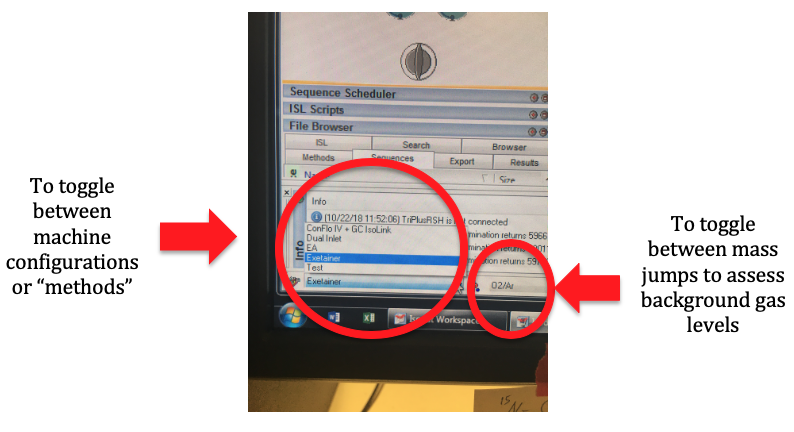
\includegraphics{/inst/img/ExetainerAnalysis/GasConfig.png}}{\# Reference gas configuration for standard exetainer analysis}}\label{reference-gas-configuration-for-standard-exetainer-analysis}
\item ~
  \subsection{Expand the ConFlo IV Diagnosis window on the left side of
  IsoDat Acquisition. Confirm that reference gas configuration matches
  the picture
  below.}\label{expand-the-conflo-iv-diagnosis-window-on-the-left-side-of-isodat-acquisition.-confirm-that-reference-gas-configuration-matches-the-picture-below.}

  \subsection[\# ]{\texorpdfstring{\#
  \protect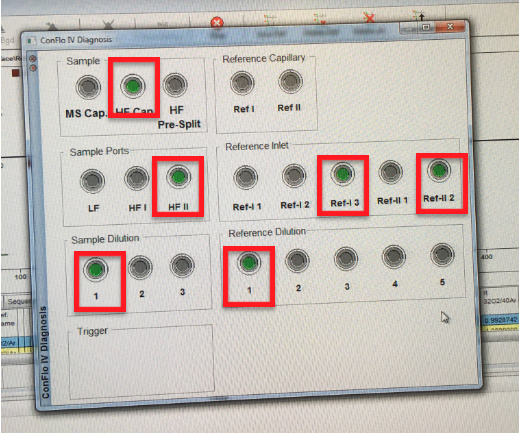
\includegraphics{/inst/img/ExetainerAnalysis/ConfloSettings.png}}{\# Reference gas configuration for standard exetainer analysis}}\label{reference-gas-configuration-for-standard-exetainer-analysis-1}
\end{enumerate}

\section{ORGANIZING YOUR RUN}\label{organizing-your-run}

\emph{A typical run starts with three air standards, with the first
discarded as a conditioner. The remaining standards are spread
throughout the run, typically placed at the beginning of each row.
Randomize the order with respect to amount of air.}\\
1. Arrange the air standards (n=9), water standards (n=2), and exetainer
samples (n=31) on the sampling block. The sampling block positions are
labeled with even numbers only. Starting at position \#2: - 3 air
standards (first air standard is conditioner) - 1 water standard -
Finish the first row with exetainer samples - Place an air standard at
the start of each subsequent row, followed by samples - Second to last
sample position should be the remaining water standard - Final sample
position is the final remaining air standard --- \#
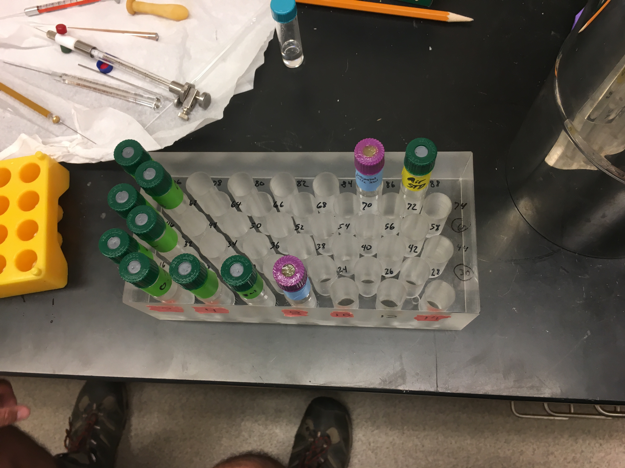
\includegraphics{/inst/img/ExetainerAnalysis/ExetainerBlock.png} ---
\emph{Note: Be aware that the numbering on the sample block does skip
some even numbers.}

\begin{enumerate}
\def\labelenumi{\arabic{enumi}.}
\setcounter{enumi}{1}
\tightlist
\item
  Take the block to the computer station to enter the standard and
  sample information into a Sequence File.\\
\item
  In IsoDat Workspace, open Exetainers\_template.seg and ``Save
  as\ldots{}'' a unique identifier for your run/sequence. This file has
  spaces for a full run.\\
\item
  In the column labeled ``Identifier 1'', enter a unique name for each
  sample and/or standard replicated 4 times. \textbf{Sample labels must
  be unique accross all batches that will be analyzed together.} For
  example, if you running four batches one of after th other, these will
  be analyzed as a group and all exetainers in that group should have a
  unique name. The first four lines should likely read ``airSTD\_0'' or
  similar and you will increment the number for as long as you are
  running. Every Exetainer is measured 4 times (thus the 4 rows). Each
  Exetainer must have a unique ID, even air standard replicates (Ex:
  airSTD\_0.2\_R1, airSTD\_0.2\_R2).\\
\item
  In the column labeled ``Comment'', identify each Exetainer as either a
  ``Conditioner'', ``Standard'', ``WaterSTD'', or ``Sample'', again
  replicating 4 times. Use only these four options.\\
\item
  In the ``Identifier 2'' column, add the amount of air added to each
  air standard (in cc or mL). This column is only used for air standards
  and \textbf{must be numeric} (i.e., 0.5 with no `cc' at the end).\\
\item
  Go back through the sequence file to make sure no rows are skipped and
  that the sample information lines up correctly with the AS field that
  identifies the position in the block. Also check that the `Amount'
  field contains the sequence 1,2,2,2 for each Exetainer. A value of 1
  tells the autosampler to move to that position.\\
\item
  Save and close the sequence file.\\
\item
  For each sample and water standard, thoroughly remove all the Apiezon
  grease on the septa using Kim wipes or paper towels. The grease will
  clog the needle. Pro tip: a microspatula is useful to efficiently
  remove all Apiezon grease.\\
\item
  Add enough new vacuum oil to the septa of every Exetainer to fill the
  indented part of the cap using the dedicated pipette. The vacuum oil
  seals the septa and lubricates the needle. Don't be stingy.\\
\item
  Place the block in the autosampler tray making sure to engage the
  alignment tabs.\\
\item
  Turn on the autosampler (black switch on rear) while holding on the
  Exetainer where the needle is resting (important, or the exetainer
  will go flying across the room). The autosampler should lift the
  needle up then undergo a quick self-check. Place the spare Exetainer
  out of the way of the autosampler.
\end{enumerate}

\section{STARTING THE RUN}\label{starting-the-run}

\begin{enumerate}
\def\labelenumi{\arabic{enumi}.}
\tightlist
\item
  Reopen working sequence file in IsoDat Acquisition.\\
\item
  If the mass spec run will include anything less than the full
  autosampler tray (i.e., running a subset of samples or a small
  sequence), highlight all the rows corresponding to the samples in the
  block.\\
\item
  Make sure that all of your desired sample rows are highlighted before
  you start the machine. NACHO will only run what has been highlighted
  in IsoDat.\\
\item
  From the drop-down menus at the top of the screen select Acquisition
  -\textgreater{} Start. \textbf{Do not hit the ``start button'' above
  the spreadsheet unless you have a full block and all rows in the
  sequence file correspond to samples.}\\
\item
  An acquisition window will appear. The application will ask you to
  name the output .xlsx. Delete the word ``acquisition'' in the file
  name for brevity. Specify the export file type as an Excel file and
  rename the export file, ending with the date in the format yyyymmdd.
\item
  Click OK to begin the run.
\item
  Wait to check that the autosampler needle has fully penetrated the
  septum of the first vial. The hexagonal nut above the needle should be
  positioned below a white plate. If it is not, you can push the needle
  down with your finger. You may have to apply more vacuum oil to
  prevent this problem from affecting further samples.
\item
  It is advisable to watch the first couple of sample injections to make
  sure everything is working properly. Specifically, you are looking for
  the presence of seven peaks of roughly equal size and the absence of a
  small pressure peak immediately after the first two reference gas
  peaks. See example chromatogram below.
\end{enumerate}

\section{VERIFYING ALL IS WELL WITH THE
RUN}\label{verifying-all-is-well-with-the-run}

After the first conditioning sample there are a couple of things you can
check to make sure that things are working as they should.\\
* If you notice a right skew in your peaks, you may need to condition or
bake the column to remove any contamination. Skewed peaks will prevent
complete peak integration before the machine moves on to the next mass
jump, rendering your data unusable.\\
* Watch for a small pressure peak soon after the second reference gas
peak. This indicates the needle is becoming clogged. If you are fast,
you can quickly clean the needle between samples.\\
* Look at the d34/32O2 of the air standards. They should range from -2.5
to -1.5. The first injection is often up around -3, but you can
disregard that. Generally, you may always disregard the data from each
first injection. * Check that the d13C is around -26.6 +/- 0.5 for
injections 2-4. This value is relative to the working standards, so
don't expect them to match known values for the real world. * At the end
of your run, check that the area for the d32-O2 curves at high and low
standard concentrations bracket the d32-O2 areas for your unknown
samples. Again, look at the 2nd or 3rd injections across vials. If they
do not, you will need to run additional air standards with a different
air range in the next batch of samples. For example, if your samples
have more O\textsubscript{2} than your highest standards, add standards
with more air in them.

\section{HELPFUL TIPS AND TIDBITS}\label{helpful-tips-and-tidbits}

\subsection{HOW TO UNCLOG THE AUTOSAMPLER
NEEDLE}\label{how-to-unclog-the-autosampler-needle}

\begin{enumerate}
\def\labelenumi{\arabic{enumi}.}
\tightlist
\item
  Ensure that the autosampler needle is not clogged before beginning
  each run. The autosampler needle will need to be unclogged if a small
  pressure peak appears after the second O\textsubscript{2}/Ar reference
  peak.\\
\item
  Turn off the autosmaples at the black switch on the back. Push the
  needle down with your finger on the white plastic block.\\
\item
  Increase the pressure of the He stream from its operational 22 psi to
  the maximum psi using the black knob at on the white box back an to
  the right of the autosampler.\\
\item
  Lift up on the needle gaurd and wipe the needle opening with a
  Kimwipe. You can also gently clear the first 1-2 mm of the inside of
  the bottom opening of any septa fragments with a small gauge needle or
  piece of wire.\\
\item
  Cover the bottom opening on the autosampler needle with a finger to
  purge the top (intake) opening, wipe with a Kimwipe, and repeat.\\
\item
  Re-adjust the pressure to of the He stream to 22 psi.\\
\item
  Turn the autsampler back on and wait for a sucessful self check.
\end{enumerate}

\section{EXAMPLE CHROMATOGRAMS}\label{example-chromatograms}

Your chromatogram should have seven peaks, shown below, in the following
order:\\
O\textsubscript{2}/Ar working standard reference peak\\
O\textsubscript{2}/Ar working standard reference peak\\
O\textsubscript{2}/Ar in your sample\\
\textbf{Mass jump}\\
N\textsubscript{2} in your sample\\
N\textsubscript{2} working standard reference peak\\
\textbf{Mass jump}\\
CO\textsubscript{2} in your sample\\
CO\textsubscript{2} working standard reference peak\\
--- \#
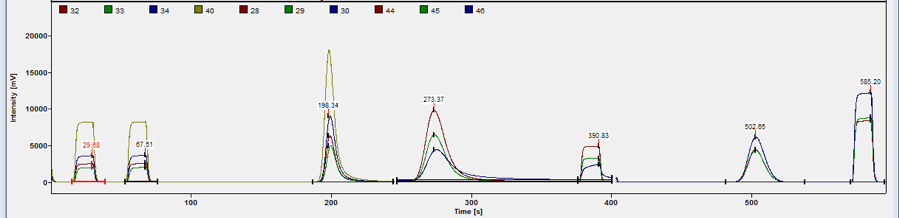
\includegraphics{/inst/img/ExetainerAnalysis/ExetainerChromatogram.png}
--- \# ENDING A RUN \& CLEAN UP Remove standards and samples from the
block. Place in a cardboard Exetainer box or rack and return to the HEEL
for cleaning and reuse. The system is ready to start another run if
desired (return to beginning of this protocol). Follow the remaining
steps if the system will remain idle for more than a couple of hours.
Place an empty Exetainer (with cap) under the needle at its home
position. Turn off the autosampler. The needle will drop down on to the
Exetainer but not puncture the septa. Align the septa under the needle
and push the autosampler needle through.\\
Lower the He carrier gas pressure (white box) from 23 psi to 5 psi. Wait
to make sure the pressure is stable at 5 psi and does not go to zero. In
IsoDat Acquisition, switch from the ``Exetainer' configuration (bottom
left pull down menu) to the ``GC-C Interface'' configuration.

\section{RETREIVING THE DATA}\label{retreiving-the-data}

\subsection{OPTION 1}\label{option-1}

\begin{enumerate}
\def\labelenumi{\arabic{enumi}.}
\tightlist
\item
  On the Desktop, open the EA\_Results folder and select the date of
  your run. These are saved using the nomenclature yymmdd. Check the
  chromatograms (.dmf files) to ensure the presence and adequate
  separation of all peaks. Check within all folders with the dates that
  apply to your mass spec run. If the IsoDat Acquisition was restarted
  due to a communication error between the IsoDat Acquisition and the
  Delta V mass spec, this will lead to multiple Excel summary files
  pertaining to your run. Copy each one to your hard drive.
\item
  Save the data to a disc. Do not transfer files using a USB; this may
  introduce viruses to this PC.
\end{enumerate}

\subsection{OPTION 2 (preferred)}\label{option-2-preferred}

\begin{enumerate}
\def\labelenumi{\arabic{enumi}.}
\tightlist
\item
  Data are dynamically backed up to the HEEL NAS system and can be
  accessed there. First, network to the following location:\\
  \href{//acoustics.washington.edu/home/CloudStation/Backup/nacho_OSB446_DellPC/G9J8G32/C/Thermo/Isodat\%20NT/Global/User/Conflo\%20II\%20Interface/Results}{//acoustics.washington.edu/home/CloudStation/Backup/nacho\_OSB446\_DellPC/G9J8G32/C/Thermo/Isodat
  NT/Global/User/Conflo II Interface/Results}
\item
  The user is HEEL, password: TreyReil1995.
\item
  Check within all folders with the dates that apply to your mass spec
  run. If the IsoDat Acquisition was restarted due to a communication
  error between the IsoDat Acquisition and the Delta V mass spec, this
  will lead to multiple Excel summary files pertaining to your run. Copy
  each one to your hard drive.
\end{enumerate}

\section{SOME THINGS TO KNOW}\label{some-things-to-know}

\begin{itemize}
\tightlist
\item
  Working standards for O\textsubscript{2}/Ar (a custom, pre-mixed
  tank), N\textsubscript{2} and CO\textsubscript{2} come from standard
  gas tanks located in the closet just beyond the computer. These tanks
  have a long life on this machine since we draw microliters at a
  time.\\
\item
  The order and number of working standard injections is by the elution
  times of the sample gases. There is no oven on this column, so we
  cannot control precisely when the sample gases elute from the column
  and the timings are sensative to room temperature.\\
\item
  We use two O\textsubscript{2}/Ar standards because 1) there is ample
  time before the O\textsubscript{2}/Ar sample elution and 2) it primes
  the machine a bit.\\
\item
  Sample data is calculated based on working standard data, which are
  verified by the air standards prepped at the beginning of this
  protocol.
\end{itemize}

\section{WASTE}\label{waste}

After your samples have been run, they need to be disposed of as
chemical waste. Exetainer samples may contain relatively dilute
concentrations of zinc chloride (ZnCl\textsubscript{2}) and have been
acidified to pH 2 with 50\% w/v H\textsubscript{3}PO\textsubscript{4}.
Exetainer caps may be thrown away; they are not reused. Collect all
liquid waste in a hazardous waste container (label suggestion below).
Exetainers should be cleaned according to the ``Exetainer Cleaning''
protocol.

\begin{longtable}[]{@{}ll@{}}
\toprule
Chemical Composition & vol \%\tabularnewline
\midrule
\endhead
Water & 99\tabularnewline
Phosphoric Acid (H\textsubscript{3}PO\textsubscript{4}) &
\textless{}1\tabularnewline
Zinc Chloride (ZnCl\textsubscript{2}) & \textless{}1\tabularnewline
\bottomrule
\end{longtable}

\begin{verbatim}
## 
## 
## ----------------------  ------------
## File rendered on:       30 Mar 2019 
## R version:              3.5.3       
## HEEL package version:   0.2.2       
## ----------------------  ------------
\end{verbatim}


\end{document}
